\scanpage{117}
\margin{N.B. On n'utilise que les \unsure{élémts de structure} 1, 2, 3}
Soit $G$ un groupe \deleted{\unsure{pro}} alg. connexe sur $Q$ provenant d'une situation motivique \inserted{$M$}, donc $U=\operatorname{Ker}(G^{\unsure{\circ|0}}\xrightarrow{\varepsilon}G_m)$. On a donc un \unsure{élément} canonique dans $\unsure{G_m}$.

\deleted{On a \unsure{$U$ sous $G$}}

\uline{Proposition} 1. Conditions équivalentes

(i) $U$ est un tore.

(ii) $\varepsilon$ est primitif dans l'ens des caractères $G^{\unsure{\circ|0}}\mathbin{-}G_m$

(iii) $M_{\mathbb R}$ admet un foncteur fibre \inserted{(``non modifié'')}, i.e. $\mathscr G_{\mathbb R}\ne\varnothing$.

\margin{\figure{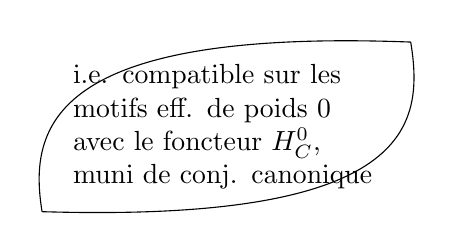
\begin{tikzpicture}
\node[align=left,text width=4cm,inner sep=8pt] (n) {i.e. compatible sur les motifs eff. de poids $0$ avec le foncteur $\unsure{H^0_{\mathbb C}}$, \unsure{muni de conj. canonique}};
\draw ([xshift=-3pt]n.south west) .. controls ([xshift=-8pt]n.west) and ([yshift=5pt]n.north west) .. (n.north east) .. controls ([xshift=5pt]n.east) and ([yshift=-4pt]n.south east) .. ([xshift=-3pt]n.south west);
\end{tikzpicture}}}
\unsure{C'est} tjs vrai si $M$ à degrés pairs, i.e. $j(\mu_2)=0$.

\uline{Proposition} 2. Conditions équivalentes

(i) $U$ est de la forme $U^{\unsure{\circ|0}}\times\mu_2$, $U^{\unsure{\circ|0}}$ un tore

(ii) $\varepsilon$ est \deleted{\unsure{un primitif}} un carré \inserted{dans $\operatorname{Hom}(G^{\unsure{\circ|0}},G_m)$}

(iii) $M_{\mathbb R}$ n'a pas de foncteur fibre \inserted{``non modifié''}, i.e. $\mathscr G_{\mathbb R}=\varnothing$.

Le fait que i) implique ii) \inserted{dans prop 1 ou prop. 2} résulte trivialt de \deleted{\unsure{l'implication de}} l'existence de $j$ avec $\varepsilon j(\lambda)=\lambda^2$, ainsi que le fait que $(1\,\mathrm{ii})\Longleftrightarrow(\text{non }\deleted{\unsure{1\,\mathrm{ii}}}\,2\,\mathrm{ii})$.

On a $(\mathrm{iii})\Rightarrow(\mathrm{ii})$, car plus précisément pour $\forall$ \deleted{\unsure{degré}} \inserted{objet} de \deleted{\unsure{degré}} \deleted{\unsure{tout}} \inserted{degré} \uline{impair} de $M_{\mathbb R}$, le \deleted{degré} \inserted{rg} doit être pair, comme il résulte de l'existence d'une forme alternée fondamentale. D'autre part i) $\Rightarrow$ (iii), car si $T$ est un tore compact sur $\mathbb R$, on a $H^{\unsure{2}}(\mathbb R,T)=0$ ! Enfin, si \deleted{\unsure{$G$}} \inserted{$M$} est à degrés pairs i.e. $j(\mu_2)=0$, donc $j=2j'$ et $\varepsilon j'=\mathrm{id}$, donc on a (ii).

\uline{Cor} Si $M$ est quelconque, la sous-catégorie \inserted{motivique} $M^{\text{pair}}$ \deleted{\unsure{satisf.}} \unsure{càd} qui correspond à $G/\deleted{\unsure{I}}j(\mu_2))$ \deleted{\unsure{est}} admet un $\mathbb R$-foncteur fibre.
\mspage{116}
